\documentclass[runningheads]{llncs}
\usepackage{amsmath}
\usepackage{booktabs}
\usepackage[compress]{cite}
\usepackage{color}
\usepackage{graphicx}
\usepackage{hyperref}

\renewcommand\UrlFont{\color{blue}\rmfamily}

\begin{document}

\title{
    Making History Count
}
\author{Gabriele Cerizza}
\authorrunning{G. Cerizza}

\institute{Università degli Studi di Milano\\
\email{gabriele.cerizza@studenti.unimi.it}\\
\url{https://github.com/gabrielecerizza/information_retrieval_project}}

\maketitle

\section{Introduction}
\label{sec:introduction}

In this report we detail our findings in the study of two tasks related to project number 9 for the Information Retrieval course of Università degli Studi di Milano.\footnote{\url{https://island.ricerca.di.unimi.it/\~alfio/shared/inforet/2020-21/inforet-projects.html}}

\section{Semantic Shifts}
\label{sec:semantic_shifts}

The first task is concerned with measuring the diachronic semantic shift or lexical semantic change (LSC) of words across time. Formally, given a set of words $W$, a word embedding function $E$ and two time periods $t_1$ and $t_2$, we want to measure
\begin{equation}
    D(w_{t_1}, w_{t_2}) = \text{distance}(E(w_{t_1}), E(w_{t_2})) \,,
\end{equation}
where $w_{t_1}$ and $w_{t_2}$ correspond to the same word $w$ used in corpora of time periods $t_1$ and $t_2$.

\subsection{Related Work}
\label{subsec:semantic_shifts:related_work}

In literature, the attempts to capture semantic shifts by way of word embeddings can be categorized in mainly two families: static embeddings or type-based models, and contextualized embeddings or token-based models.

\subsubsection{Static Embeddings Models.} Static embeddings represent each word with a single vector. This vector can be considered a summarization of the occurrences of a word in different contexts. Popular static embeddings are obtained from skip-gram with negative sampling (SGNS)~\cite{mikolov-etal-2013-word2vec}, GloVe~\cite{pennington-etal-2014-glove} and fastText~\cite{bojanowski-etal-2017-fasttext}.

We could train two models on corpora of different time periods and then measure the cosine distance between the embeddings of a given word. The issue in this direct comparison is that SGNS and the other neural models are stochastic in nature and may produce embeddings that are differently rotated along the axes (invariance under rotation). Common solutions include:

\begin{itemize}
    \item orthogonal Procrustes method, which aligns the embeddings to the same coordinate axes~\cite{hamilton-etal-2016-diachronic,prazak-etal-2020-uwb}, but may introduce noise in the projections~\cite{dubossarsky-etal-2019-time, zhou-li-2020-temporalteller};
    \item initialization of the weights of one model with the weights of the other model, which can be problematic for new words~\cite{kutuzov-etal-2018-diachronic,tahmasebi-etal-2018-survey};
    \item second-order similarity, which first computes the similarity of a word to other words in one vector space, then computes the similarity of the same word to other words in the other vector space, and finally compares the two similarities~\cite{kutuzov-etal-2018-diachronic,tahmasebi-etal-2018-survey}.   
\end{itemize}

\subsubsection{Contextualized Embeddings Models.} Recently developed neural models like BERT~\cite{devlin-etal-2018-bert} generate different word embeddings for each different context (sentence) in which a word appears. 

Contextualized embeddings models start by extracting a vector for each occurrence of a word. Then, these models cluster the vectors of the two periods to find the different senses of a word. After that, they measure how the frequency of the senses changed between the time periods to get an estimate of the semantic shift~\cite{giulianelli-etal-2020-analysing,rother-etal-2020-cmce}. An alternative approach computes the average pairwise distance between each vector of one period and each vector of the other period~\cite{laicher-etal-2021-explaining,pomsl-lyapin-2020-circe,kutuzov-giulianelli-2020-uio}.  
 

\subsection{Proposed Methods}
\label{subsec:semantic_shifts:methods}

\subsubsection{Orthogonal Procrustes Method (OP).} We started by collecting pretrained static word embeddings. For the historical corpus we used the embeddings provided in~\cite{sprugnoli-tonelli-2019-histo}. These embeddings were trained with fastText on documents dated 1860-1939 and taken from the Corpus of Historical American English (COHA\footnote{\url{https://corpus.byu.edu/coha/}}), for a total of 198M tokens. For the contemporary corpus we used fastText word embeddings trained on Wikipedia and news\footnote{\url{https://fasttext.cc/docs/en/english-vectors.html}} for a total of 16B tokens.

Considering the size of the contemporary vocabulary, as well as the fact that it contained misspelled words, we decided to analyze only the 5000 most frequent words in the contemporary vocabulary, intersected with the historical vocabulary. We also included the “target" words indicated by SemEval-2020~\cite{schlechtweg-etal-2020-semeval} for evaluation purposes (see Subsection~\ref{subsec:semantic_shifts:results}).

Finally, we aligned the vectors with orthogonal Procrustes and computed the cosine distance between the two embeddings of each selected word.

\subsubsection{Nearest Neighbors Method (NN).} This approach leverages ideas taken from the second-order similarity techniques over static embeddings. We used the same word embeddings and selected the same words as described for OP.

For each selected word we took the 15 nearest neighbors in the historical vector space; then we measured the cosine distance between the word and these neighbors in the historical vector space; after that, we measured the cosine distance between the word and the same neighbors, but in the contemporary vector space; finally, we computed the mean squared error (MSE) between the distances measured in the historical vector space and the distances measured in the contemporary vector space. Then we did the same for the 15 nearest neighbors in the contemporary model. Finally, we took the mean between the two MSE. 

We shrunk the vocabulary of the two models to their intersection to guarantee that each neighbor found in one vector space was also present in the other. 

\subsubsection{Jensen-Shannon Distance Method (JSD).} This method is based on contextualized embeddings. The corpora were taken from SemEval-2020~\cite{schlechtweg-etal-2020-semeval}. The historical corpus contained shuffled sentences from 1810-1860, while the contemporary corpus contained shuffled sentences from 1960-2010. Both corpora were composed of 6M tokens.

We analyzed the 5000 most frequent words in both corpora, keeping only adjectives, nouns and verbs. We filtered stop words and tokens containing non-alphabetic characters. We aggregated the embeddings according to lemma and POS tags. Our assumption is that the semantic shift of a word is invariant to declension and conjugation.

We generated the embeddings from BERT. We fine-tuned the transformer on the historical corpus for 5 epochs. Note that we used only one model to generate embeddings for both time periods. Since BERT generates different embeddings for different contexts, it suffices that BERT acquired knowledge of the contexts used in both time periods~\cite{martinc-etal-2020-leveraging}. For the embeddings, we took only the hidden state of the last layer, which is reportedly the layer most related to semantics~\cite{laicher-etal-2021-explaining}.

Following the approach described in~\cite{rother-etal-2020-cmce}, we first employed an autoencoder and UMAP~\cite{mcinnes-2020-umap} to reduce the dimensionality of the embeddings from 768 to 10. The combination of autoencoder and UMAP was shown to be effective for clustering in~\cite{mcconville-etal-2019-n2d}. Then, we clustered the embeddings of a given word with HDBSCAN, which is a variant of DBSCAN with improved robustness and a single hyperparameter~\cite{campello-etal-2013-hdbscan}. 

Interpreting the clusters as senses of a word, we measured the frequency of each sense in the two time periods. Finally, we used the Jensen-Shannon distance to measure the similarity between the two senses distributions.

\subsection{Results}
\label{subsec:semantic_shifts:results}

In Table~\ref{tab:semantic_shifts:top_words} we show the 10 words with most semantic shift according to the proposed methods. OP identified many words whose meaning changed due to technological evolution, like “cd", “tv" and “bot". OP and NN also captured shifts of historical or cultural nature, like “isis" and “gay". The semantic shifts detected by JSD are not as readily decipherable.

\begin{table}
    \caption{Top 10 words with the most semantic shift detected by the methods.}
    \label{tab:semantic_shifts:top_words}
    \centering
    \begin{tabular}{lll}
        \toprule
        OP & NN & JSD \\
        \midrule
        cd & deletion & negro (adj.) \\
        romney & km & people (noun) \\
        km & gay & golf (noun) \\
        diff & diff & shopping (noun)  \\
        deletion & outstanding & overall (adj.) \\
        tv & implement & businessman (noun) \\
        template & highlight & switch (verb) \\
        isis & parameter & investor (noun) \\
        bot & red & motor (noun) \\
        highlight & template & user (noun) \\
        \bottomrule
    \end{tabular}
\end{table}

In Figure~\ref{fig:semantic_shifts:score} we give an example of how the shift in senses was perceived by the JSD method. We can see, for instance, that the verb “score" assumed a meaning more related to sports as the time passed.

\begin{figure}
    \center
    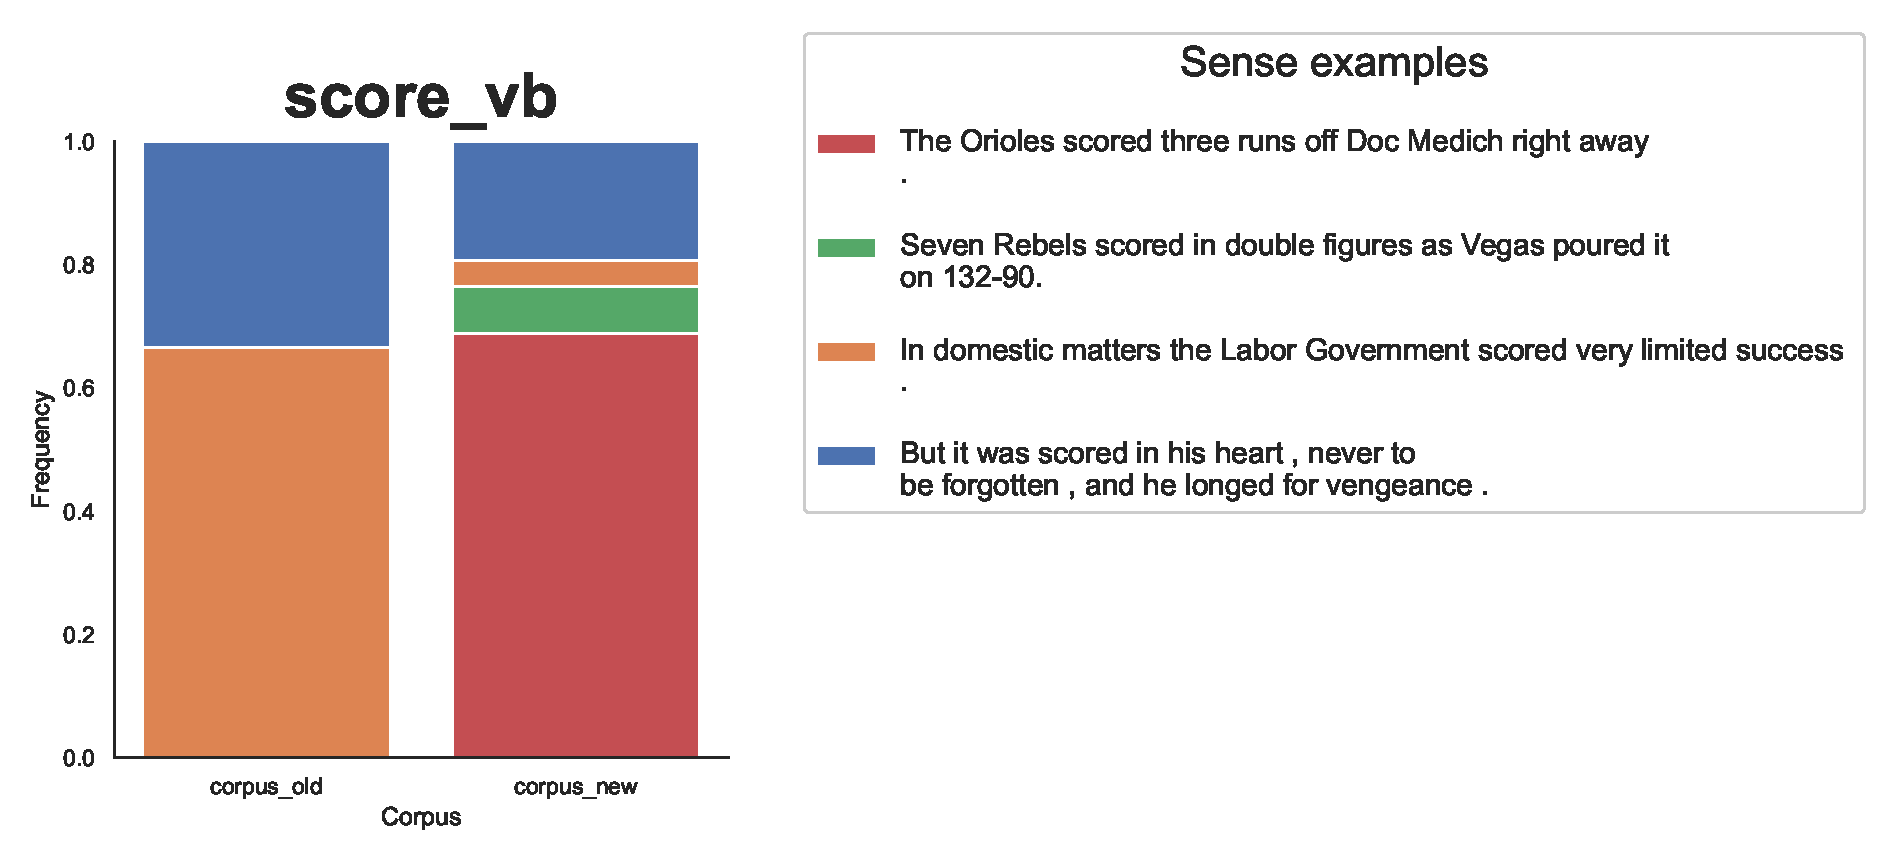
\includegraphics[width=1\textwidth]{img/33_score_vb.eps}
    \caption{Shift in the frequency of senses for the verb “score".} 
    \label{fig:semantic_shifts:score}
\end{figure}

Furthermore, we evaluated our results against a ground truth for the semantic shift occurred in 37 words provided by SemEval-2020~\cite{schlechtweg-etal-2020-semeval}. In Table~\ref{tab:semantic_shifts:spearman} we compare the Spearman's rank-order correlation of our methods with the top 5 systems in the SemEval-2020 shared task. We deduce that our methods are competitive with other state-of-the-art systems.

\begin{table}
    \caption{Spearman's rank-order correlation to SemEval-2020 ground truth for the proposed methods and the top systems in the competition.}
    \label{tab:semantic_shifts:spearman}
    \centering
    \begin{tabular}{|c|c|c|c|c|c|c|c|}
        \toprule
        OP & NN & JSD & UG\_Student\_Intern & Jiaxin \& Jinan & cs2020 & UWB & Discovery\_Team \\
        \midrule
        .391 & .341 & .365 & \textbf{.422} & .325 & .375 & .367 & .361 \\
        \bottomrule
    \end{tabular}
\end{table}

\subsection{Conclusion}
\label{subsec:semantic_shifts:conclusion}

Tables~\ref{tab:semantic_shifts:top_words} and~\ref{tab:semantic_shifts:spearman} suggest that static embeddings methods perform slightly better than contextualized embeddings methods. The same conclusion can be found in literature~\cite{laicher-etal-2021-explaining,schlechtweg-etal-2020-semeval}. Possible reasons for this behavior are the small size of the corpora for the JSD method and a need of further fine-tuning. Another possible reason lies in the fact that the historical corpus contains a lot of artifacts.

A possible improvement in the JSD method involves tuning the HDBSCAN hyperparameter to find a number of senses for each word that is similar to the number of word synsets found in WordNet.

\section{Historical Event Extraction}
\label{sec:historical_events}

The second task involves the detection of historical events in a text and the extraction of the event arguments, such as dates, historical figures and locations. The Histo Corpus described in~\cite{sprugnoli-tonelli-2019-histo} was suggested for this task. The event recognition model was to be evaluated on Wikipedia pages.

\subsection{Definition of Historical Event}

The notion of “historical event" is not clearly defined. Since “individuation criteria are not given by nature or language"~\cite{shaw-2010-phdthesis}, ultimately the choice of what constitutes an historical event is arbitrary. Here we consider historical such events and entities that may be the subject of a paragraph in a history textbook. These primarily concern military and political occurrences, which is consistent with~\cite{cybulska-vossen-2011-historical}.

\subsection{Data Sets}

The Histo Corpus is composed of news and travel narratives from 1865-1926 and is annotated with events, consisting mainly in verbs and participles. Three issues prevented us from using this corpus. 

\begin{enumerate}
    \item The corpus is “historical" in the sense that the documents are not contemporary, but the annotated events are not “historical" in the sense that they are not characterized by historical figures or by episodes that we may find in a history textbook. 
    \item Since the corpus is annotated with “common" events described using a “historical" language, we would have no way to recognize “historical" events described using a “contemporary" language in Wikipedia.
    \item The annotations are limited to the events themselves and do not include arguments, like dates and people involved in the events.
\end{enumerate}

To the best of our knowledge, there are no public English data sets in which historical events are annotated along with their arguments. A promising data set, described in~\cite{lai-etal-2021-event}, is yet to be published as of the time of this writing.

For the recognition of events and their arguments, we employed the RAMS data set~\cite{ebner-etal-2020-rams}, in which 139 event types, each with up to 5 arguments, were annotated. Each document contains 5 sentences. The arguments of an event may be found in different sentences from the one in which the event is mentioned.

We also built a data set composed of 1024 pages taken from Wikipedia, for a total of 4M tokens. Each page was classified as historical or not based on the properties of the corresponding Wikidata entry. Each page was split into paragraphs to which we assigned the same class of the page. By exploiting the links in the text and Wikidata, we likewise classified the entities mentioned in each paragraph as historical or not. Finally, each paragraph was annotated in the BIO format with the Wikipedia entities mentioned therein.

\subsection{Strategy}

We adopted the following strategy. First, we built a model to classify a given paragraph as historical or not. We make the assumption that Wikipedia pages related to historical entities are more likely to describe historical events in their paragraphs. Note that we cannot base our classification solely on the entities mentioned in a paragraph, because: (i) the link to an entity is usually provided only for the first mention; (ii) the surface form of an entity can vary greatly.

Once the paragraphs related to historical events were identified, other models were employed to extract the event and the pertaining arguments.

\subsection{Related Work}

Formally, the event extraction problem can be stated as follows. We define an ontology of event types $t \in T$, each of which is associated with a set of $n_t$ arguments $A_t$. Given a document $d = \langle w_1, \dots, w_m \rangle$, we want to find which event $t$, if any, is described in $d$, possibly identifying the event “trigger" word, and which words correspond to the $n_t$ arguments of the event $t$, if any.    

We categorize the models found in literature in two families: span classification approaches and machine reading comprehension (MRC) approaches.

\subsubsection{Span Classification Approaches.} These approaches group words in spans and exploit event and argument annotations to assign labels to each span. There are methods that learn embeddings for each span, possibly adding external features such as POS tags and dependencies in the parser tree, and then use a neural network~\cite{ebner-etal-2020-rams,zhong-chen-2021-frustratingly,nguyen-nguyen-2019-one-for-all} or transformers~\cite{chen-etal-2020-joint-modeling} to classify each span. Some methods also employ graphs within the process~\cite{lin-etal-2020-oneie,wadden-etal-2019-entity,luan-etal-2019-general,nguyen-2021-gcn}. 

\subsubsection{MRC Approaches.} These approaches do not label spans, but rather produce a natural language response to a natural language prompt. There are models that fill placeholders in a predefined template with spans extracted from the text~\cite{chen-etal-2020-manual,li-etal-2021-genarg}. Other models treat the problem as a question answering task~\cite{du-cardie-2020-event,feng-etal-2020-probing,liu-etal-2020-mrc} or as a textual entailment task~\cite{feng-etal-2020-probing}. Other models yet use sequence-to-structure text generation~\cite{lu-etal-2021-text2event}.

\subsection{Proposed Methods}

\subsubsection{Paragraph Classification.} We adopted a multi-task learning model (MTL) to classify paragraphs as historical or not. First, we obtained BERT embeddings for each token. Then, we used two feed-forward neural networks (FFNN) to jointly learn (i) the paragraph class, and (ii) the tag of the entities referenced in the paragraph. Cross-entropy loss was computed separately for each task and then summed according to learned weights~\cite{kendall-etal-2017-mtl-loss}.

We compared our model with a BiLSTM classifier and a BERT classifier.

\subsubsection{Event and Argument Extraction.} To identify events, we followed the span classification approach described in~\cite{zhong-chen-2021-frustratingly}. After enumerating all spans up to 3 tokens long, we obtained embeddings for each span by aggregating the BERT embeddings of the tokens. Then, we passed the embeddings through a FFNN to classify each span either as an event type $t$ or as a non-event. We used cross-entropy loss.

For argument extraction, we followed the MRC approach described in~\cite{li-etal-2021-genarg,wen-etal-2021-resin}. We fed a BART~\cite{lewis-etal-2020-bart} model with the paragraph and an event template with an “\textlangle{}arg\textrangle{}"  placeholder for each argument. After training, the model learned to generate the same template with the placeholders filled with text spans. We restricted the language vocabulary to that of the input during generation. We tried the same approach also for document-level event identification (EventGen).

We were unable to perform event and argument extraction jointly due to hardware constraints, so we provided the argument model with the gold event type during training. We compared our model with results reported in literature and with BiLSTM and BERT document-level classifiers.

\subsection{Results}

In Table \ref{tab:historical_events:classification} we show the results for the paragraph classification task. Table \ref{tab:historical_events:event-arguments} compares the performances on the event and argument extraction tasks. Note that the authors employed different training settings, such as using gold argument spans and gold event types or considering the syntactical head-words (most representative tokens) of the arguments instead of the whole spans, making it difficult to directly compare the models.

\vspace*{-3mm}

\begin{table}
    \caption{Accuracy (Acc), precision (P), recall (R) and F1-score for the paragraph classification task on the test set. We reported weighted average scores.}
    \label{tab:historical_events:classification}
    \centering
    \begin{tabular}{lcccc}
        \toprule
        Model & Acc & P & R & F1\\
        \midrule
        MTL & \textbf{84.2} & \textbf{80.6} & \textbf{84.2} & \textbf{82.4} \\
        BiLSTM & 74.4 & 74.7 & 74.4 & 74.5 \\
        BERT & 73.0 & 76.4 & 73.0 & 74.7 \\
        \bottomrule
    \end{tabular}
\end{table}

\vspace*{-10mm}

\begin{table}
    \caption{Precision (P), recall (R) and F1-score on the official test set of the RAMS data set. TCD stands for type-constrained decoding and refers to the practice of considering only the top-scoring $n_t$ arguments for an event type $t$ with $n_t$ arguments. For our event models we reported the weighted average scores, while for the argument model we reported the metrics computed according to the official RAMS scorer.}
    \label{tab:historical_events:event-arguments}
    \centering
    \resizebox{0.8\textwidth}{!}{
    \begin{tabular}{lccccccc}
        \toprule
        & Gold Arg. Spans & \multicolumn{3}{c}{Events} & \multicolumn{3}{c}{Arguments} \\
        Model & & P & R & F1 & P & R & F1\\
        \midrule
        Ebner et al.~\cite{ebner-etal-2020-rams} & Yes & - & - & - & 62.8 & \textbf{74.9} & 68.3 \\
        Ebner et al. (TCD)~\cite{ebner-etal-2020-rams} & Yes & - & - & - & 78.1 & 69.2 & 73.3 \\
        Zhang et al.~\cite{zhang-etal-2020-two} & Yes & - & - & -  & 71.5 & 66.2 & 68.8 \\
        Zhang et al. (TCD)~\cite{zhang-etal-2020-two} & Yes & - & - & -  & 81.1 & 66.2 & 73.0 \\
        Wei et al.~\cite{wei-etal-2021-trigger} & Yes & - & - & - & \textbf{82.0} & 71.6 & \textbf{76.6} \\
        \hline
        Li et al.~\cite{li-etal-2021-genarg} & No & - & - & - & - & - & 48.6 \\
        Zhang et al.~\cite{zhang-etal-2020-two} & No & - & - & -  & - & - & 40.1 \\
        Zhang et al. (TCD)~\cite{zhang-etal-2020-two} & No & - & - & -  & - & - & 41.8 \\
        Wen et al.~\cite{wen-etal-2021-resin} & No & - & - & - & - & - & 48.6 \\
        Wei et al.~\cite{wei-etal-2021-trigger} & No & - & - & - & 53.1 & \textbf{42.7} & 47.4 \\
        Lai et al.~\cite{lai-etal-2021-event} & No & \textbf{71.9} & 74.7 & \textbf{73.2} & - & - & - \\
        Pouran Ben Veyseh et al.~\cite{pouran-ben-veyseh-etal-2021-unleash} & No & 55.5 & \textbf{78.6} & 65.1 & - & - & - \\
        Our BiLSTM baseline & No & 0.1 & 2.3 & 0.2 & - & - & - \\
        Our BERT baseline & No & 1.1 & 1.7 & 1.1 & - & - & - \\
        \textbf{Our model (EventGen)} & No & 29.8 & 27.9 & 24.8 & - & - & - \\
        \textbf{Our model} & No & 2.2 & 2.9 & 2.3 & \textbf{62.7} & 42.0 & \textbf{50.3} \\
        \bottomrule
    \end{tabular}
    }
\end{table}

\vspace*{-10mm}

\subsection{Conclusion}

With regard to the paragraph classification task, our MTL model outperforms the baseline methods. Further improvement can be attained with a more fine-grained analysis of the Wikidata properties of each Wikipedia page.

Our event model struggles to correctly identify trigger words. One reason is that the vast majority of the spans do not contain events and, therefore, finding the correct event span and the correct event type becomes a highly imbalanced problem. The EventGen model fares better and the predictions show that in many cases the mistakes were semantically close to the gold labels. Our argument model compares favourably with the baseline methods. We could improve the model by appending argument type constraints to the templates~\cite{li-etal-2021-genarg, shwartz-etal-2020-unsupervised}.

\bibliographystyle{splncs04}
\bibliography{bibtex_entries}

\end{document}